\documentclass[tikz]{standalone}
%\usetikzlibrary{calc}
\begin{document}


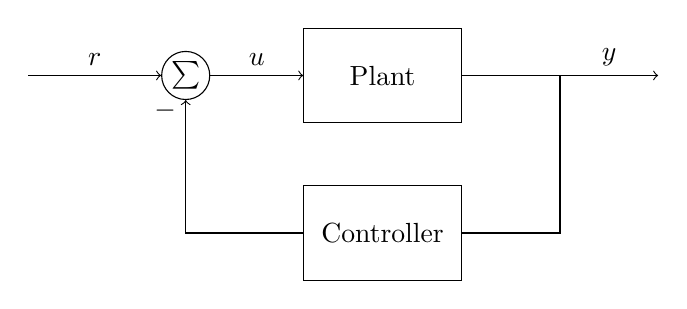
\begin{tikzpicture}[node distance=2cm, block/.style={rectangle, draw, minimum height=12mm, minimum width=20mm}, sumnode/.style={circle, draw, inner sep=1pt}]
  \node[coordinate] (input) {};
  \node[sumnode, right of=input] (sum) {$\sum$};
  \node[block,right of=sum, node distance=25mm] (plant) {Plant};
  \node[block,below of=plant, node distance=20mm] (controller) {Controller};
  \node[coordinate, right of=plant, node distance=35mm] (output) {};

  \draw[->] (input) -- node[above] {$r$} (sum);
  \draw[->] (sum) -- node[above] {$u$} (plant);
  \draw[->] (plant) -- node[coordinate] (feedback) {} node[near end, above] {$y$} (output);
  \draw[->] (feedback) |- (controller) -| (sum) node[left, pos=0.96] {$-$};

\end{tikzpicture}
\end{document}
